\clearpage

\subsubsection{Long term}
\label{subsubsec:long-res}

Since some error occurred in the indexing phase when performing the submitted runs fr\_1 and fr\_2, in the following analysis we will use a \emph{fixed} version of those runs.

In Table~\ref{tab:long-map-ndcg-table} are reported the \ac{nDCG} and \ac{MAP} values obtained from the submitted runs on the long term collection, while in Figure~\ref{fig:precision-recall-curve-long-term} is reported the interpolated Precision-Recall curve. Comparing these results with the ones obtained on the short term, shown in Table~\ref{tab:short-map-ndcg-table} and Figure~\ref{fig:precision-recall-curve-short-term} respectively, we can see that every run suffered a \emph{performance drop} over all the measures. This worsening was expected and it can be due to the fact that the performances tend to drop over time, however, the decrease is not huge and we can consider the performances of the system to \emph{remain satisfactory}.

Observing the \ac{nDCG} and \ac{AP} boxplots, shown in Figure~\ref{fig:long-boxplot}, we can notice that the runs performed on the French collection have a similar structure in terms of median values and interquartile ranges. We can also notice that in the \ac{AP} boxplot all the runs show the presence of outliers. 

From the ANOVA2 analysis, which results are reported in Table~\ref{tab:long-anova2}, we can see that we obtained very different results for the two measures. In particular, on \ac{nDCG} we have $p\textrm{--}value>\alpha$, which means we \emph{cannot reject} the null hypothesis, while on \ac{AP} we have $p\textrm{--}value<\alpha$, which means we \emph{can reject} the null hypothesis. The same behavior is reflected in Tukey's \ac{HSD} multiple comparison, shown in Figure~\ref{fig:long-hsd}, where on \ac{nDCG} we can derive that the French runs can be considered to be similar to each other, while on \ac{AP}  we can see that runs fr\_1, fr\_2, fr\_3 and runs fr\_3, fr\_4 can be considered similar to each other.

\begin{table}[tbp]
\caption{\ac{nDCG} and \ac{MAP} values on long term collection}
  \label{tab:long-map-ndcg-table}
    \centering
    \begin{tabular}{|p{0.7\linewidth}|p{0.075\linewidth}|p{0.075\linewidth}|}
	\toprule
	\textbf{Run name} & \textbf{nDCG} & \textbf{MAP} \\
	\midrule
        FADERIC\_French-BM25-Stop50-LightStem-Shingle-Fuzzy-SynCustom-Rerank20W6 & 0.4153 & 0.2473 \\ 
        FADERIC\_French-BM25-Stop50-LightStem-Shingle-Fuzzy-Rerank30 & 0.4146 & 0.2465 \\ 
        FADERIC\_French-BM25-Stop50-LightStem-Shingle-Fuzzy-SynCustom & 0.4091 & 0.2384 \\ 
        FADERIC\_French-BM25Tuned-Stop50-LightStem-Shingle-Fuzzy & 0.4071 & 0.2350 \\ 
        FADERIC\_English-BM25-Stop50-KStem-Shingle-Fuzzy-SynPOS\\-Rerank30 & 0.3296 & 0.1809 \\ 
	\bottomrule
    \end{tabular}
\end{table}

\begin{figure}[tbp]
  \centering
  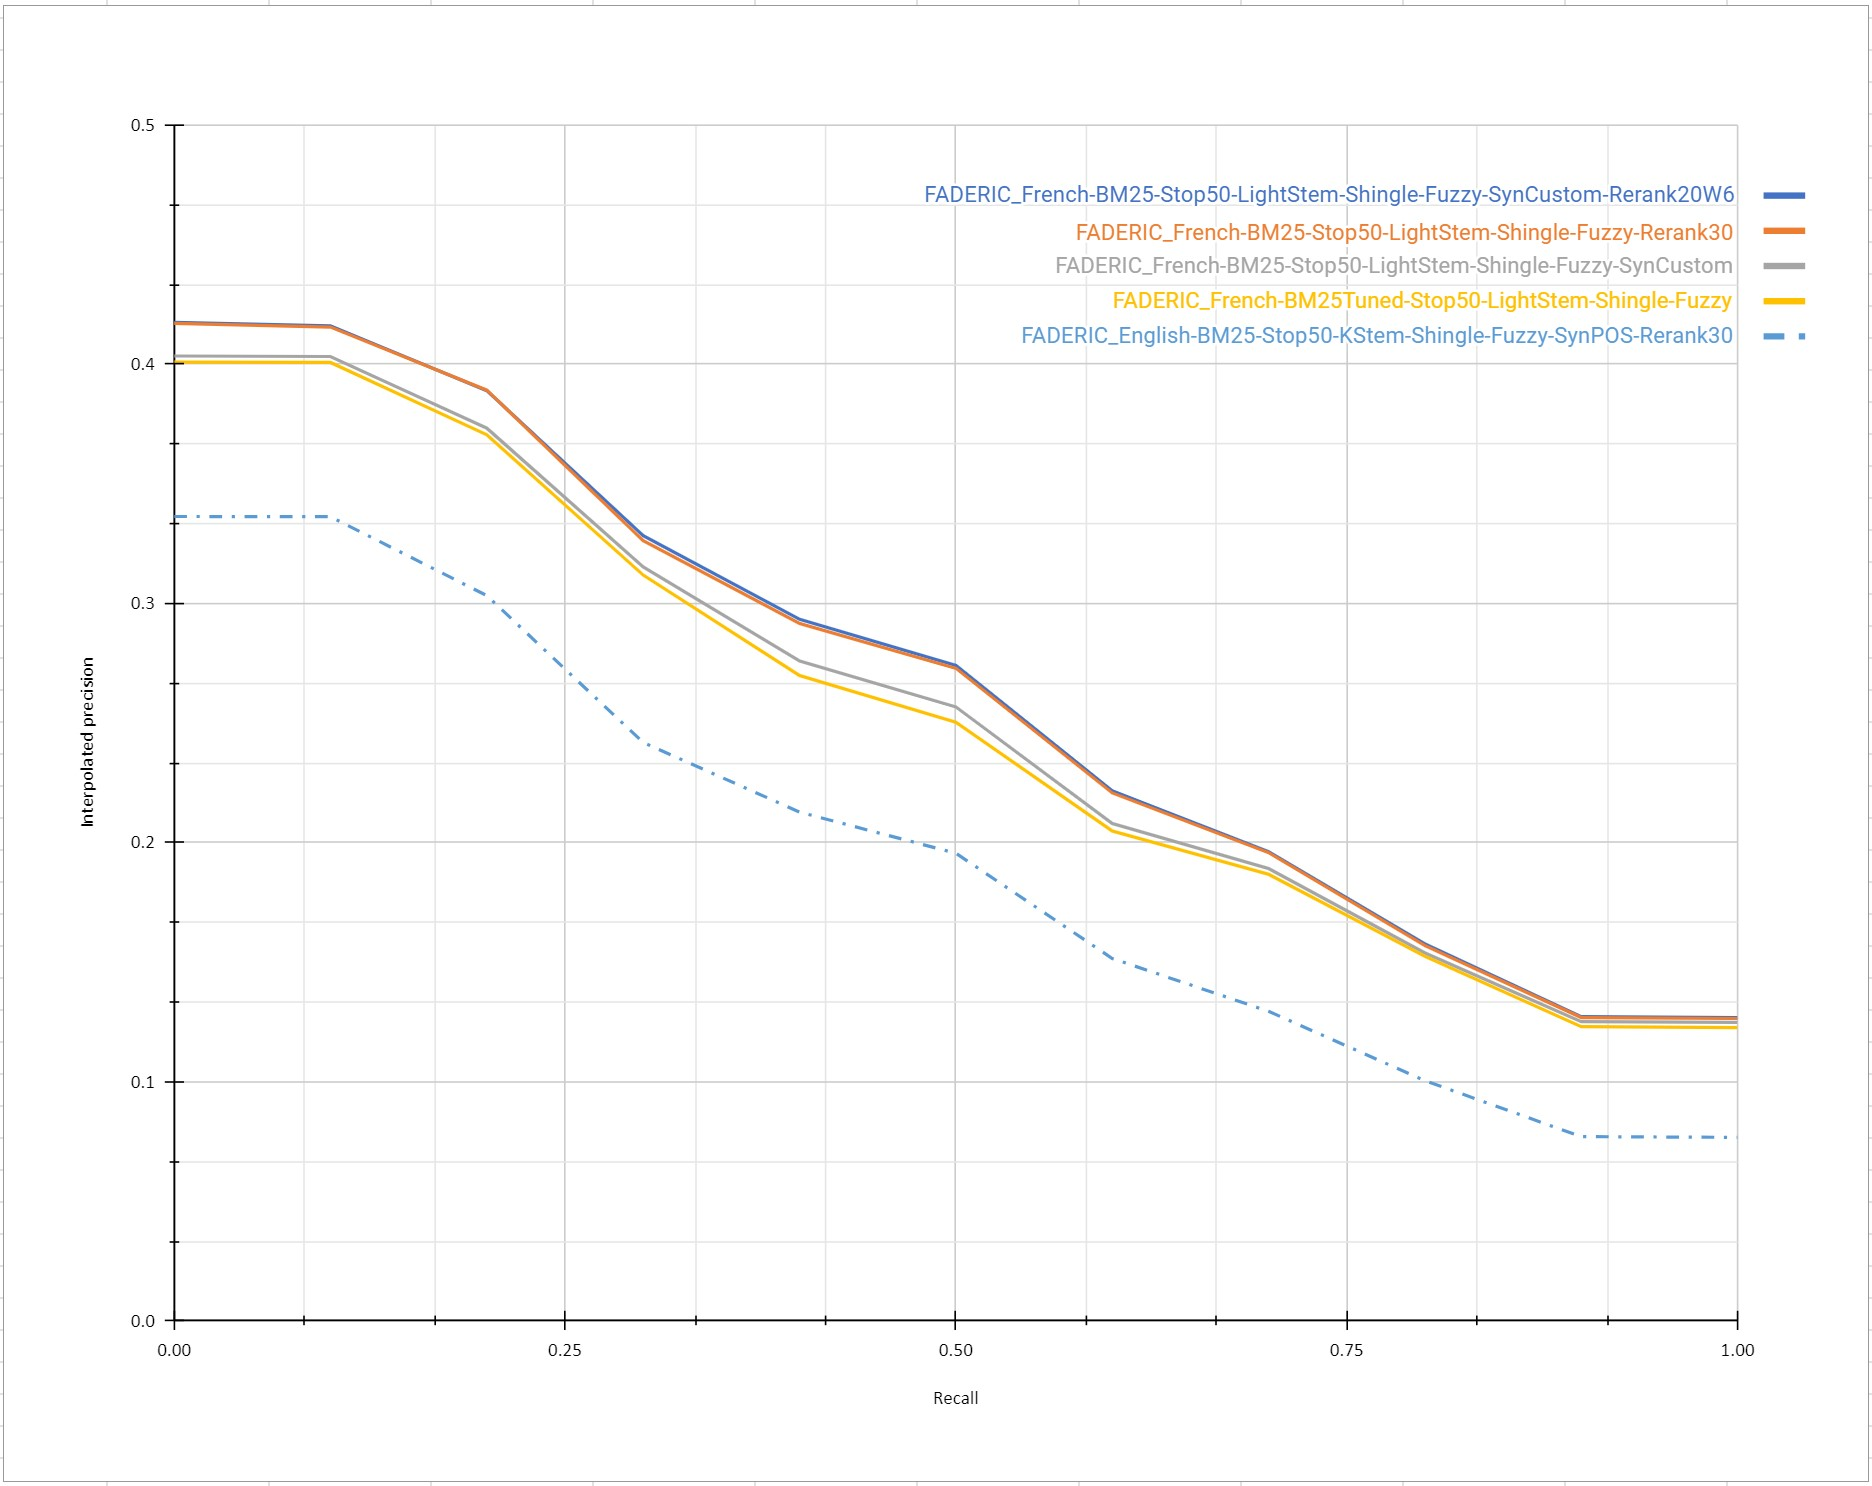
\includegraphics[width=1\linewidth]{figure/iprec-recall-LONG-TERM.jpg}
  \caption{Interpolated Precision-Recall curve on long term collection}
  \label{fig:precision-recall-curve-long-term}
\end{figure}

\begin{figure}[tbp]
     \centering
     \begin{subfigure}[b]{0.45\textwidth}
         \centering
         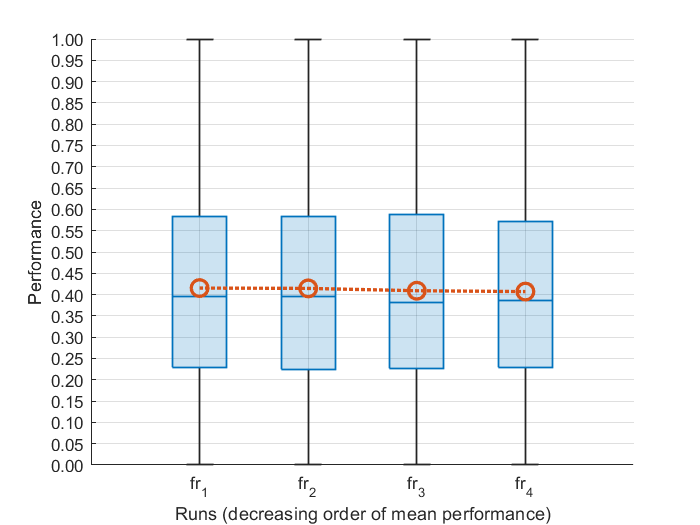
\includegraphics[width=\textwidth]{figure/long-ndcg-boxplot.png}
         \caption{\ac{nDCG}}
     \end{subfigure}
     \hfill
     \begin{subfigure}[b]{0.45\textwidth}
         \centering
         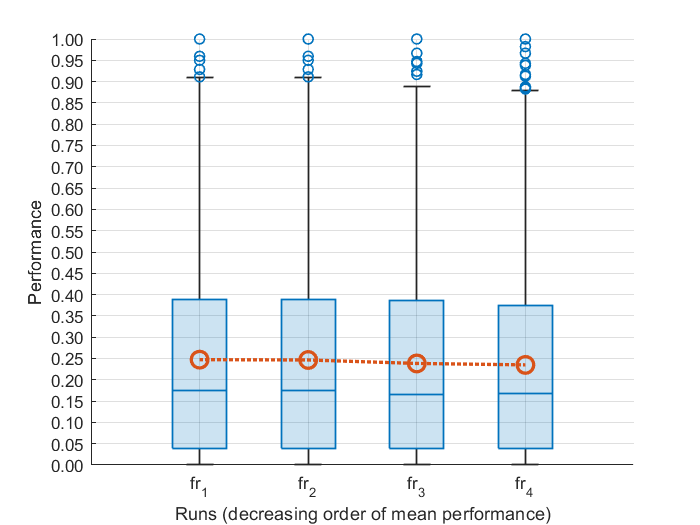
\includegraphics[width=\textwidth]{figure/long-map-boxplot.png}
         \caption{\ac{AP}}
     \end{subfigure}
        \caption{Box plot on long term collection, the mean values are shown in red}
        \label{fig:long-boxplot}
\end{figure}

\begin{table}[tbp]
     \caption{ANOVA2 on long term collection}
    \begin{subtable}[h]{1\textwidth}
        \centering
	\caption{\ac{nDCG}}
        \begin{tabular}{|l|l|l|l|l|l|}
	\toprule
        \textbf{Source} & \textbf{SS} & \textbf{df} & \textbf{MS} & \textbf{F} & \textbf{Prob$>$F} \\
        \midrule
	\textbf{Systems} & 0.04 & 3   & 0.015  & 1.51  & 0.056 \\
	\textbf{Topics}    & 202.35  & 922  & 0.219 & 16.17 & 0 \\
	\textbf{Error}   & 16.78  & 2766 & 0.006 & - & - \\
	\textbf{Total}   & 219.18  & 3691 & - & - & - \\
	\bottomrule
       \end{tabular}
    \end{subtable}
        \begin{subtable}[h]{1\textwidth}
        \centering
	\caption{\ac{AP}}
        \begin{tabular}{|l|l|l|l|l|l|}
	\toprule
        \textbf{Source} & \textbf{SS} & \textbf{df} & \textbf{MS} & \textbf{F} & \textbf{Prob$>$F} \\
        \midrule
	\textbf{Systems} & 0.10 & 3   & 0.033  & 4.47  & 0.003 \\
	\textbf{Topics}    & 188.61  & 922  & 0.204 & 27.03 & 0 \\
	\textbf{Error}   & 20.92  & 2766 & 0.007 & - & - \\
	\textbf{Total}   & 209.64  & 3691 & - & - & - \\
	\bottomrule
       \end{tabular}
    \end{subtable}
     \label{tab:long-anova2}
\end{table}

\begin{figure}[tbp]
     \centering
     \begin{subfigure}[b]{0.4\textwidth}
         \centering
         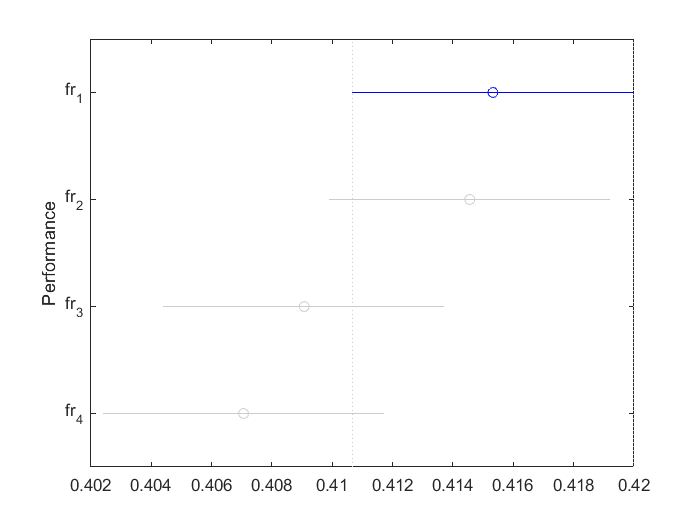
\includegraphics[width=\textwidth]{figure/long-ndcg-hsd.png}
	\caption{\ac{nDCG}}
     \end{subfigure}
     \hfill
     \begin{subfigure}[b]{0.4\textwidth}
         \centering
         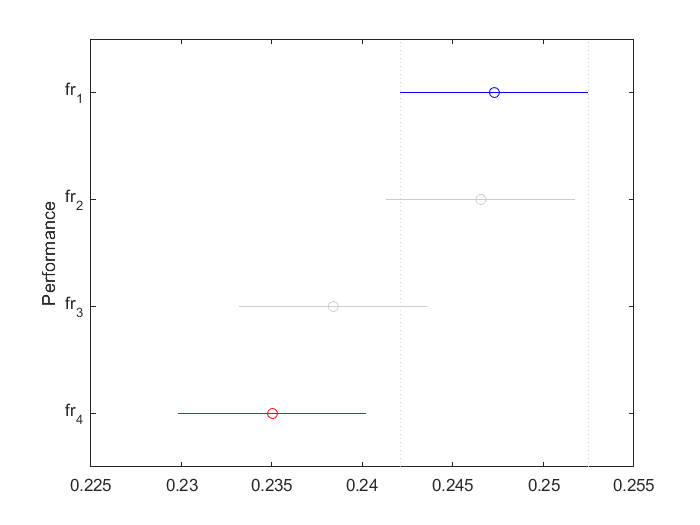
\includegraphics[width=\textwidth]{figure/long-map-hsd.png}
	\caption{\ac{AP}}
     \end{subfigure}
        \caption{Tukey's \ac{HSD} on long term collection}
        \label{fig:long-hsd}
\end{figure}